
Continuous relations have \emph{infinitely many} points.
So it's impossible to describe the relation as a set of ordered pairs, since you would have 
to write down an infinite number of pairs.
Similarly, we cannot write the domain or range as sets of ordered pairs.
We need a different way to do it.

\begin{myConceptSteps}{To find the domain of a continuous relation\dots}
    \myStep{the curve}{Look closely at the curve.}
    \myStep{$x$ coordinates}{Ask yourself \,``What are the $x$ coordinates of the points on the curve?''}
    \myStep{left-to-right}{Describe those $x$ coordinates as you go from left to right. That description is the domain.}
\end{myConceptSteps}

Mathematicians use \emph{inequalities} or \emph{interval notation} in their descriptions of the domain.
You will learn this in the examples.

\begin{myExample}{
    Find the domain of this relation.
    \begin{center}
        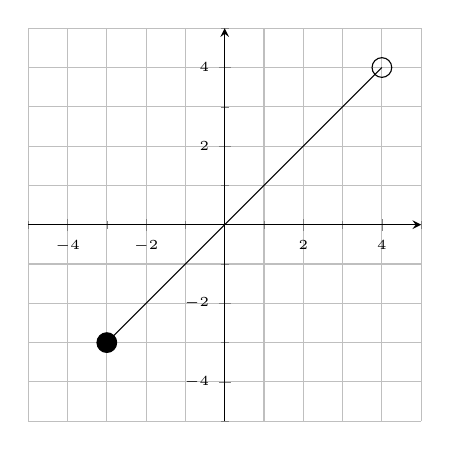
\begin{tikzpicture}
            \begin{axis}[
                width=3in,
                grid=both,
                axis x line = middle,axis y line = middle,
                axis equal image,
                xtick distance = 2, ytick distance = 2, 
                minor tick num = 1,
                xmin = -5, xmax=5,
                ymin = -5, ymax=5,
                tick label style = {font=\tiny},
                ]
                \addplot[mark=*,mark size=0.125cm,] coordinates { (-3,-3) };
                \addplot[mark=o,mark size=0.125cm,] coordinates { (4,4) };
                \addplot[no marks, samples=100, domain=-3:4, ] expression { x };
            \end{axis}
        \end{tikzpicture}
    \end{center}
}
    \vspace{1.75in}
\end{myExample}

\begin{myExample}{
    \begin{center}
        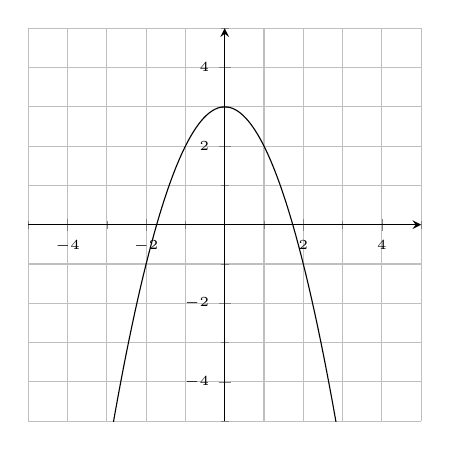
\begin{tikzpicture}
            \begin{axis}[
                width=3in,
                grid=both,
                axis x line = middle,axis y line = middle,
                axis equal image,
                xtick distance = 2, ytick distance = 2, 
                minor tick num = 1,
                xmin = -5, xmax=5,
                ymin = -5, ymax=5,
                tick label style = {font=\tiny},
                ]
                \addplot[no marks, samples=100, domain=-3:4, ] expression { -x^2 + 3 };
            \end{axis}
        \end{tikzpicture}
    \end{center}
}
    \vspace{1.75in}
\end{myExample}
